% !TEX encoding = UTF-8 Unicode
\documentclass{article}

\usepackage{multirow}
\usepackage[bottom]{footmisc}
\usepackage{url}
\usepackage{hyperref}
\usepackage{xepersian}
\usepackage{ulem}


\settextfont{XB Zar}

\renewcommand{\footnoterule}{
	\hrule width 3in
}
\rightfootnoterule

\title{\textbf{گام اول پروژه درس تحلیل و طراحی سیستم‌ها}}

\author{سید پارسا میرطاهری - ۹۵۱۰۹۳۹۴ \\ کیارش گل‌زردی - ۹۵۱۰۵۸۵۱}

\begin{document}

\date{}

\maketitle

\section{پروژهٔ نخست: سامانهٔ مزایدهٔ کالای برخط}

\subsection{توصیف پروژه}

هدف این پروژه ارائهٔ یک بستر برخط برای به مزایده گذاشتن کالا است. این بستر در قالب یک سیستم اطلاعاتی مبتنی بر وب طراحی می‌شود که در آن افراد قادر هستند کالاهای خود را با یک مبلغ پایه برای مدت محدودی به مزایده بگذارند. در ادامه افراد دارای حساب کاربری می‌توانند تا سقف اعتباری که حساب کاربری خود را شارژ کرده‌اند روی جنس قیمت بگذارند (در این صورت اعتبارشان برای خرید رزرو می‌شود). در پایان مدت زمان مزایده فردی که بالاترین قیمت را پیشنهاد کرده است به عنوان برندهٔ مزایده به فرد آگهی دهنده معرفی می‌شود و پس از تایید تحویل کالا توسط خریدار مبلغ قرارداد به حساب فروشنده واریز می‌شود.

\subsection{\lr{Economical Feasibility Analysis}}

\begin{center}

\begin{figure}[htp]
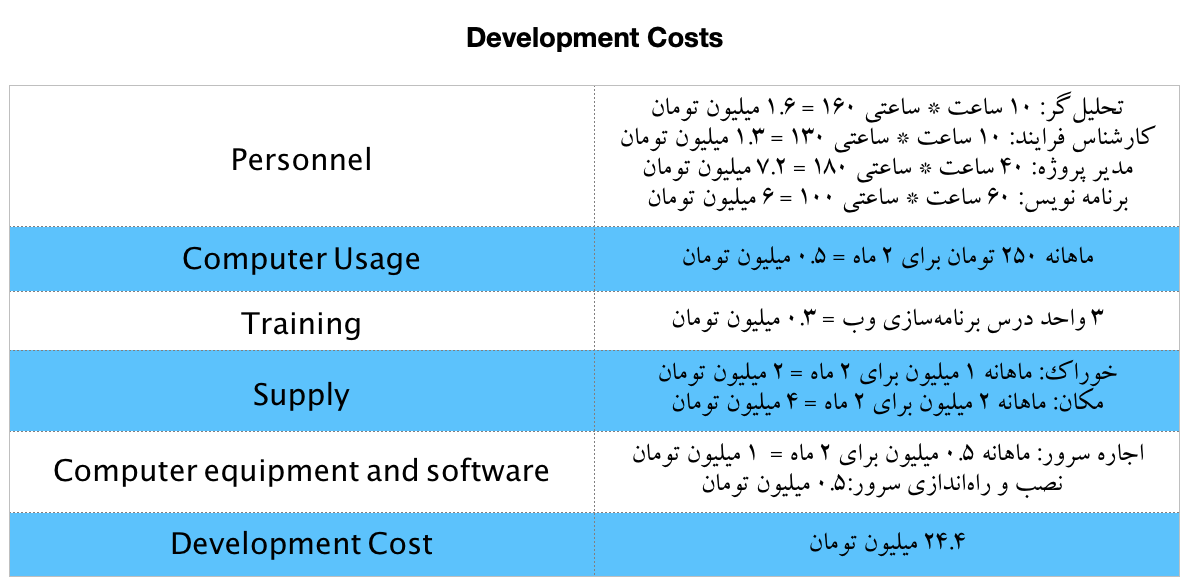
\includegraphics[width = 1\textwidth]{Dev1.png}
\caption{\lr{Developement Costs}}
\label{dev1}
\end{figure}

\begin{figure}[htp]
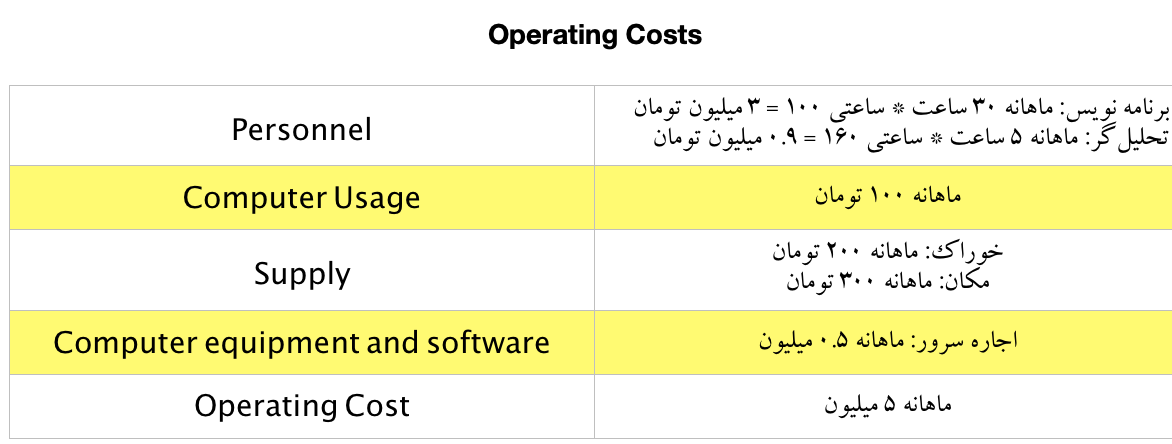
\includegraphics[width = 1\textwidth]{Op1.png}
\caption{\lr{Operating Costs}}
\label{op1}
\end{figure}

\begin{figure}[htp]
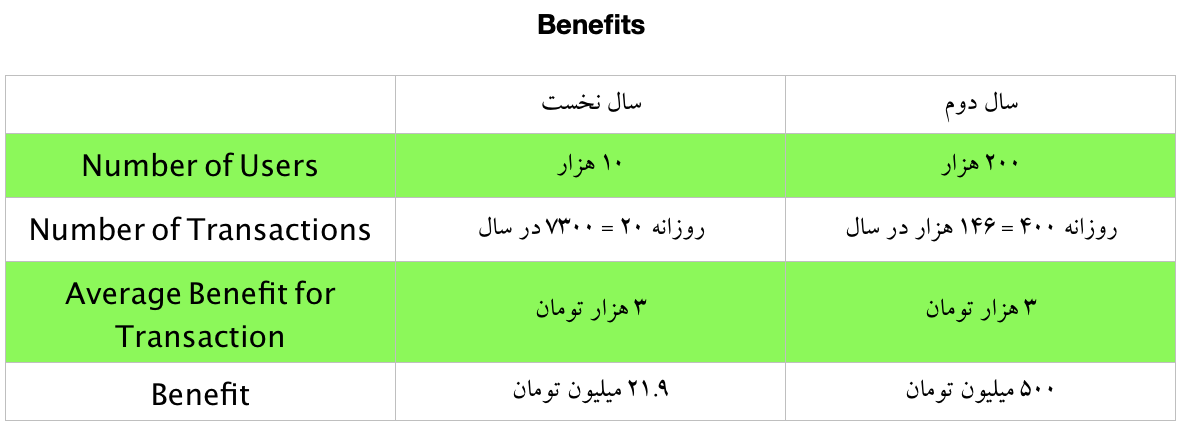
\includegraphics[width = 1\textwidth]{Ben1.png}
\caption{\lr{Benefits}}
\label{ben1}
\end{figure}

\begin{figure}[htp]
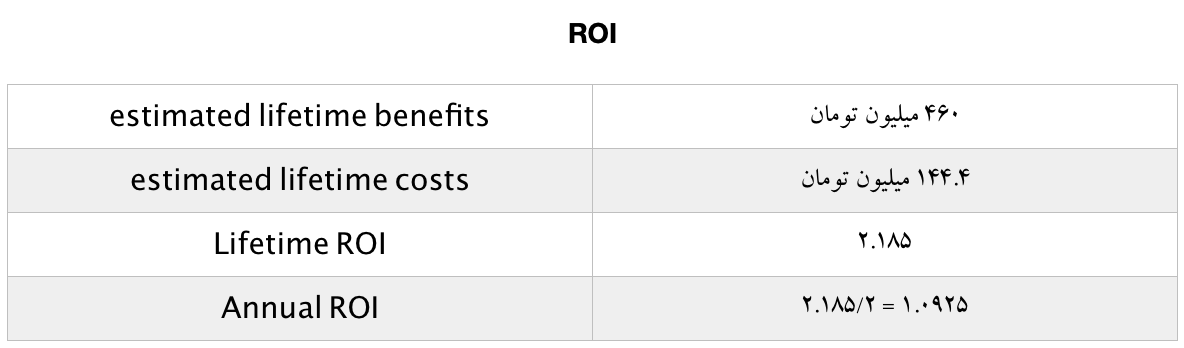
\includegraphics[width = 1\textwidth]{ROI1.png}
\caption{\lr{Return-On-Investment Analysis}}
\label{roi1}
\end{figure}

\begin{figure}[htp]
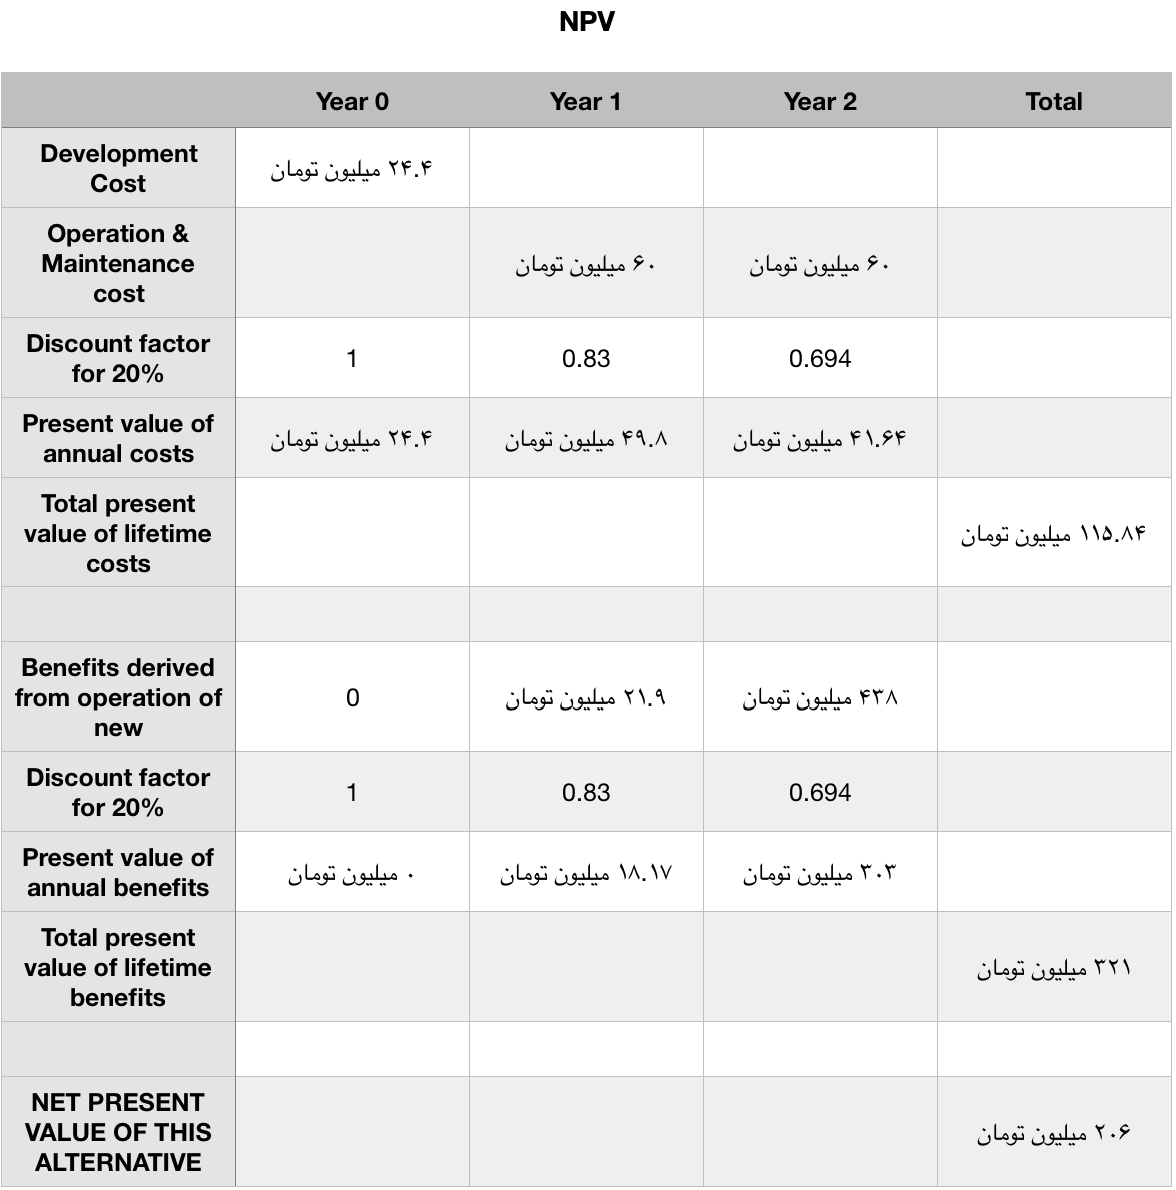
\includegraphics[width = 1\textwidth]{NPV1.png}
\caption{\lr{Net Present Value Analysis}}
\label{npv1}
\end{figure}

\begin{figure}[htp]
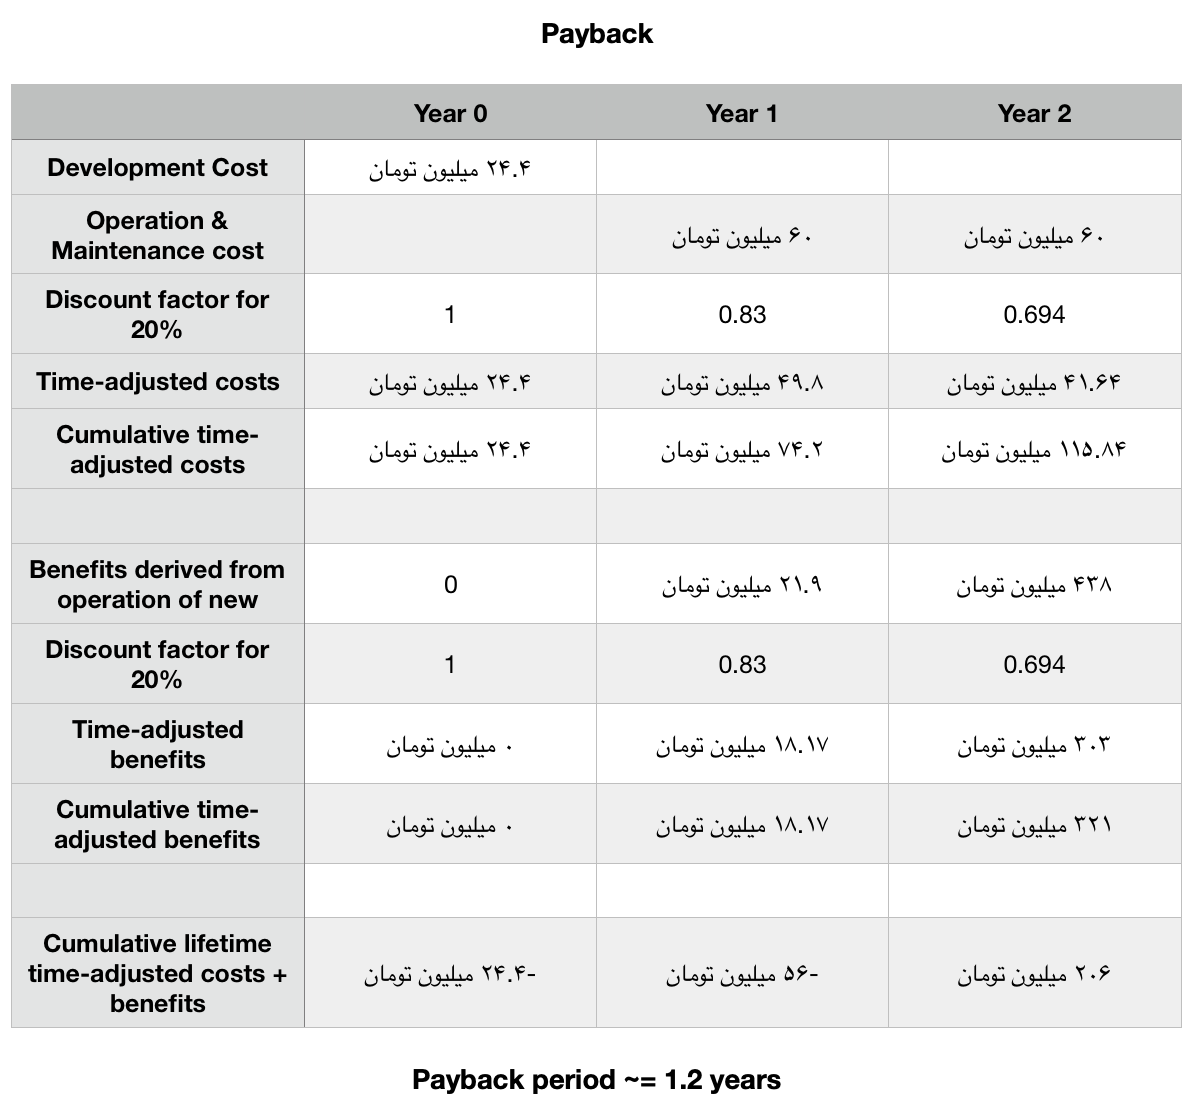
\includegraphics[width = 1\textwidth]{PB1.png}
\caption{\lr{Payback Analysis}}
\label{pb1}
\end{figure}

\end{center}

\subsection{\lr{Schedule Feasibility Analysis}}

در این پروژه همان‌طور که در بخش \ref{dev1} آمده است در بخش Developement به ۱۲۰ ساعت وقت نیاز است که نصف آن به برنامه‌نویسی اختصاص یافته و نیمهٔ دیگر آن به تحلیل، مدیریت فرایند و مدیریت پروژه اختصاص یافته است. با توجه به اینکه فرایندهایی نظیر تحلیل را می‌توان پیش از بازهٔ دوماههٔ توسعه انجام داد، این حجم از کار نزدیک به میزان توانایی و وقت تیم دونفره است و از این نظر با کمی فشار امکان‌پذیر به نظر می‌رسد.

\section{پروژهٔ دوم: سامانهٔ قرض دادن کالای برخط}

\subsection{توصیف پروژه}

هدف این پروژه ارائهٔ یک بستر برخط برای قرض دادن و قرض گرفتن کالاست. به این شکل که در قالب یک سرویس تحت وب افراد می‌توانند اجناس خود را با تعیین مبلغ پرداختی و مبلغ بیعانه برای قرض دادن قرار می‌دهند. افرادی که حساب کاربریشان به اندازهٔ مبلغ مجموع شارژ دارد می‌توانند برای قرض گرفتند اقدام کنند. سپس مبلغ کسر می‌شود و پس از تحویل کالا پیش‌پرداخت با کسر مبلغ واسطه‌گری به حساب فرد قرض دهنده منتقل می‌شود. در انتها نیز پس از پس دادن کالا و اعلام فرد قرض دهنده باقی مبلغ به قرض دهنده منتقل شده و بیعانه خریدار نیز آزاد می‌شود.

\subsection{\lr{Economical Feasibility Analysis}}

\begin{center}

\begin{figure}[htp]
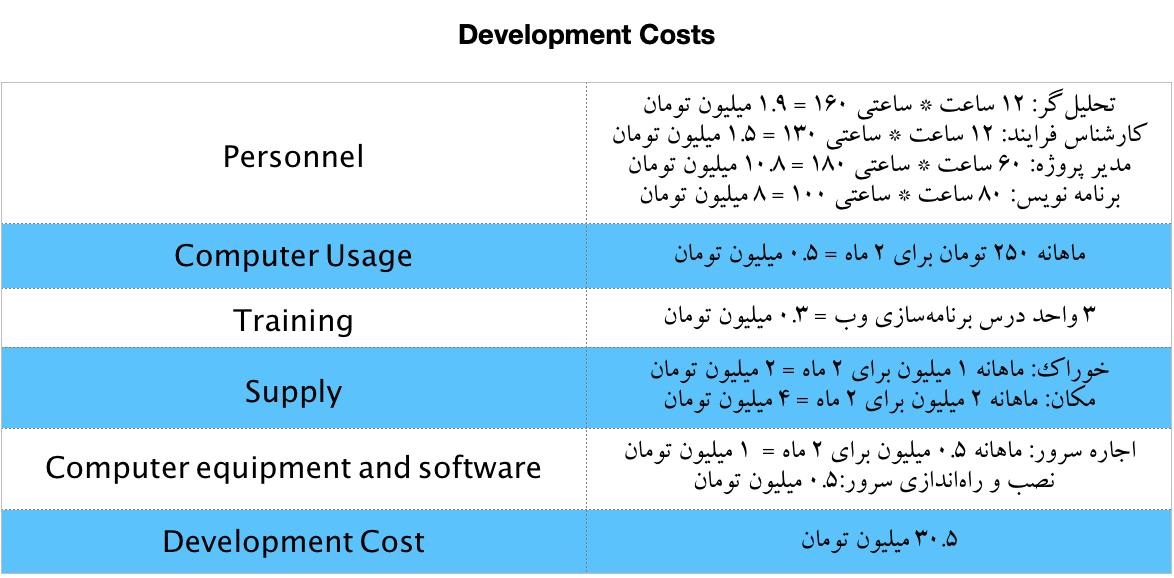
\includegraphics[width = 1\textwidth]{Dev2.png}
\caption{\lr{Developement Costs}}
\label{dev2}
\end{figure}

\begin{figure}[htp]
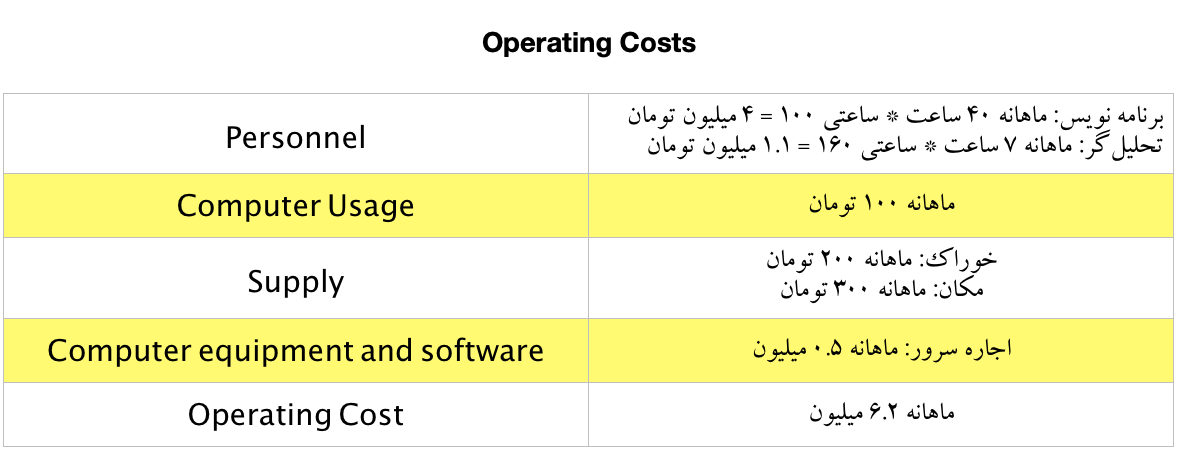
\includegraphics[width = 1\textwidth]{Op2.png}
\caption{\lr{Operating Costs}}
\label{op2}
\end{figure}

\begin{figure}[htp]
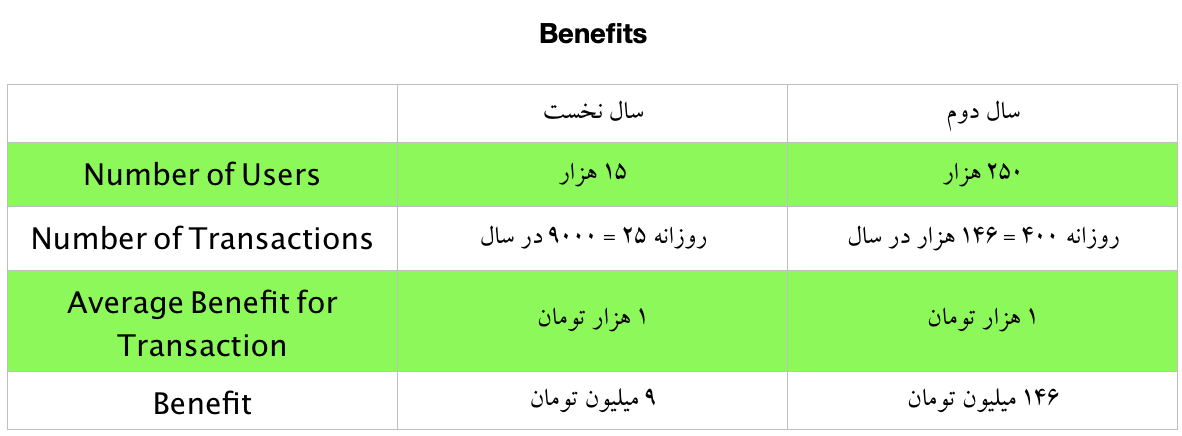
\includegraphics[width = 1\textwidth]{Ben2.png}
\caption{\lr{Benefits}}
\label{ben2}
\end{figure}

\begin{figure}[htp]
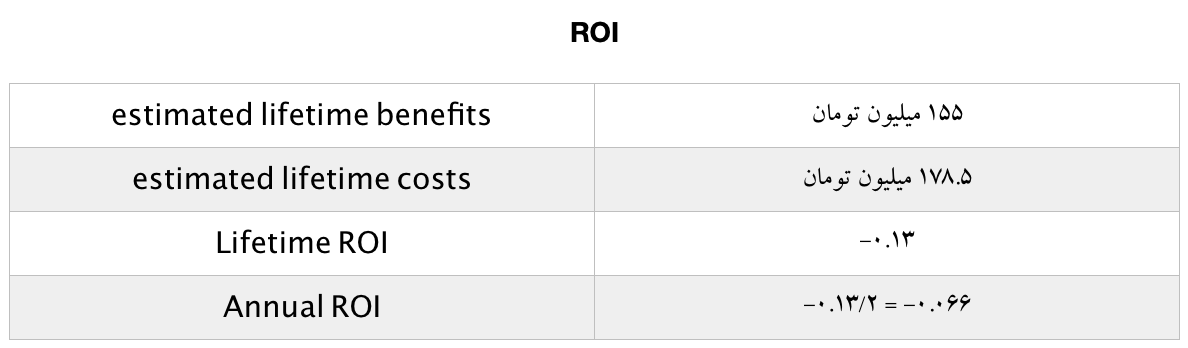
\includegraphics[width = 1\textwidth]{ROI2.png}
\caption{\lr{Return-On-Investment Analysis}}
\label{roi2}
\end{figure}

\begin{figure}[htp]
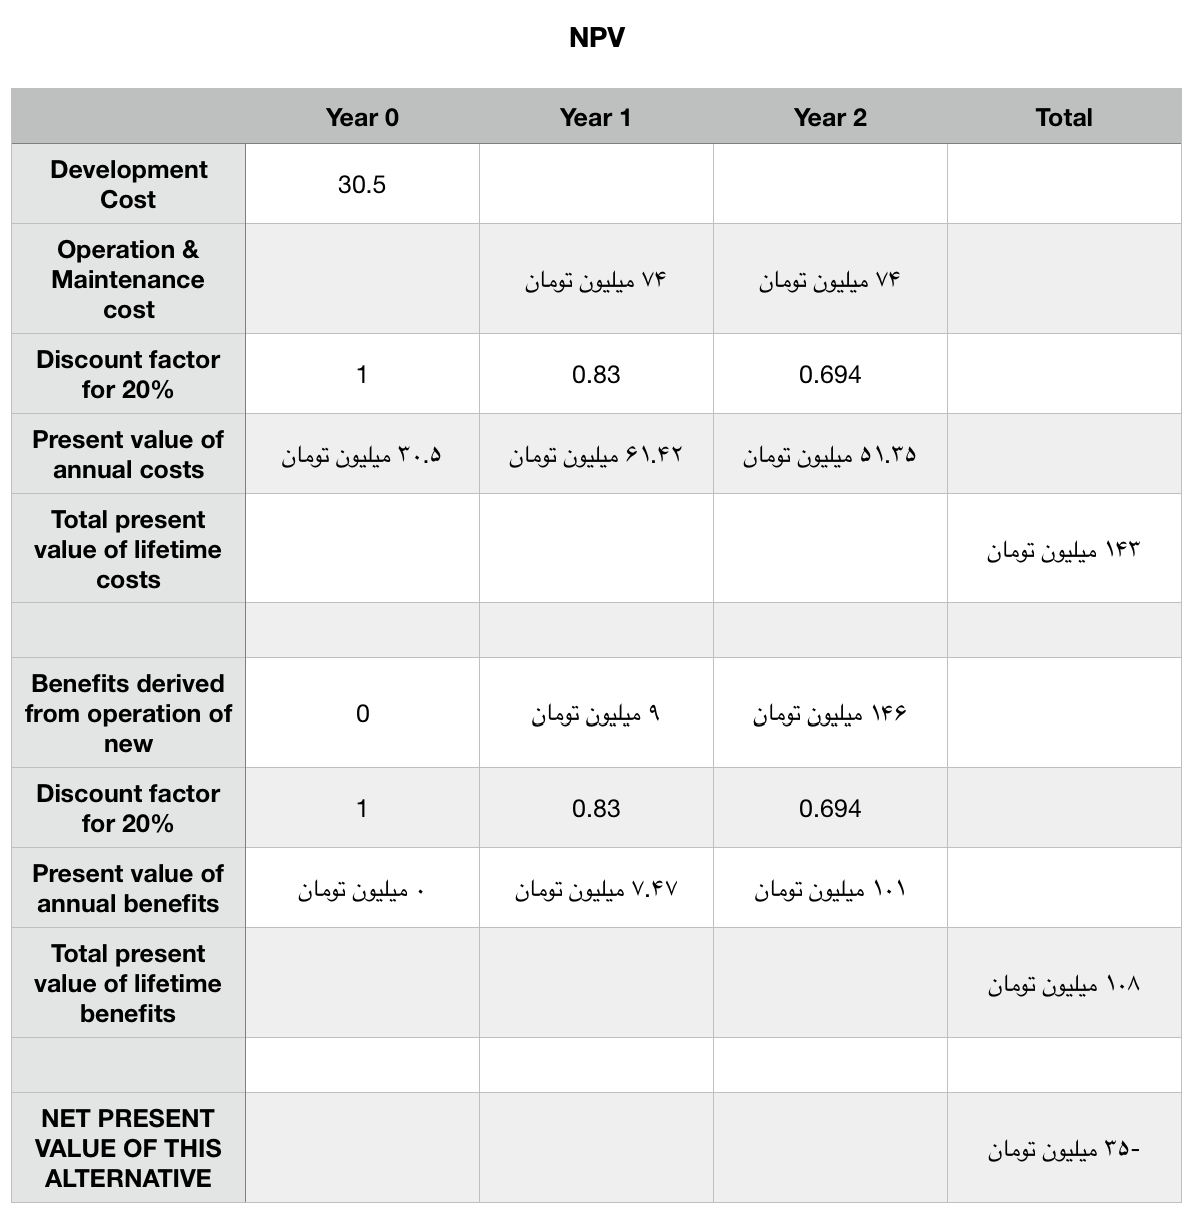
\includegraphics[width = 1\textwidth]{NPV2.png}
\caption{\lr{Net Present Value Analysis}}
\label{npv2}
\end{figure}

\begin{figure}[htp]
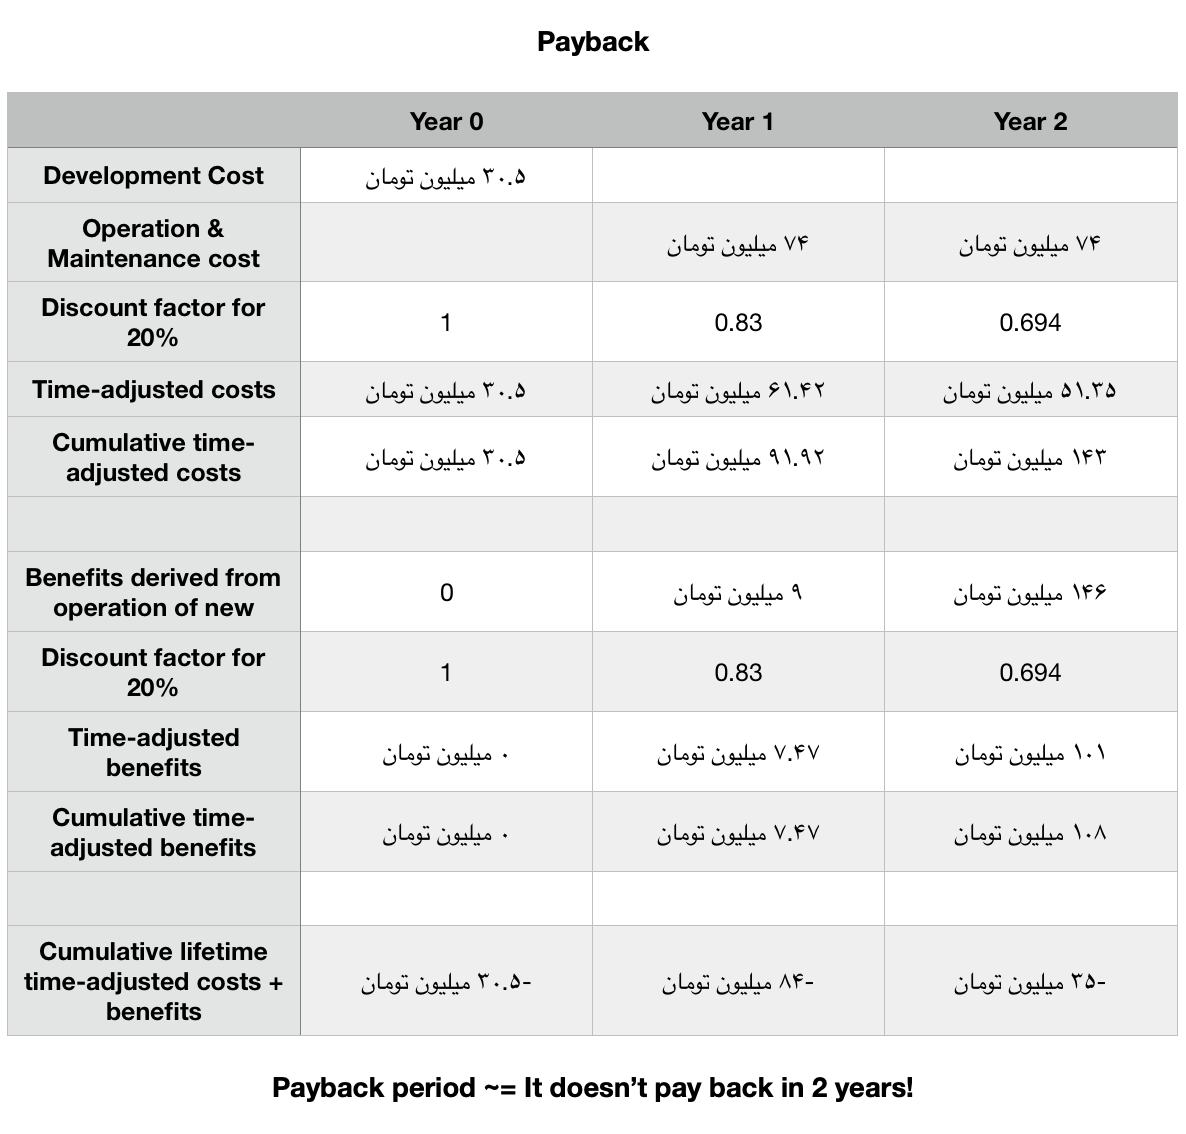
\includegraphics[width = 1\textwidth]{PB2.png}
\caption{\lr{Payback Analysis}}
\label{pb2}
\end{figure}

\end{center}

\subsection{\lr{Schedule Feasibility Analysis}}


در این پروژه همان‌طور که در بخش \ref{dev2} آمده است در بخش Developement به ۱۶۴ ساعت وقت نیاز است که تقریبا نصف آن(۸۰ ساعت) به برنامه‌نویسی اختصاص یافته و نیمهٔ دیگر آن به تحلیل، مدیریت فرایند و مدیریت پروژه اختصاص یافته است. بنا بر بررسی‌های توانایی و وقت دو نفر عضو تیم این میزان از حجم کار از وقت و توانایی تیم خارج است و در طول دو ماه چندان امکان‌پذیر به نظر نمی‌رسد.


\section{انتخاب پروژه}

خوشبختانه یا متاسفانه با تحلیل امکان‌سنجی اقتصادی و برنامه‌ای دو پروژهٔ فوق این نتیجه حاصل می‌شود که پروژهٔ دوم با وجود پیچیدگی بیشتر و به تبع آن زمان توسعه و هزینهٔ بیشتر سود کمتری را به ارمغان می‌آورد و حتی در طول دو سال به سوددهی نمی‌رسد. در نتیجه بنابر تحلیل امکان‌سنجی از نظر اقتصادی و برنامه‌ای پروژهٔ نخست، \textbf{سامانهٔ مزایدهٔ کالای برخط}، به عنوان پروژهٔ نهایی انتخاب شد. این پروژه زمان نسبتا زیادی برای توسعه می‌طلبد اما با مدیریت بهینه قابل انجام به نظر می‌رسد و از نظر اقتصادی نیز طبق بررسی‌های فوق توجیه‌پذیر به نظر می‌رسد.\\

\section{تدوین \lr{Work Breakdown Structure}}

خروجی WBS اولیه پروژه به ضمیمه آمده است.\\

\end{document}
